\documentclass[11pt]{article}
\usepackage{amsfonts}
\usepackage{amsmath}
\usepackage[makeroom]{cancel}
\usepackage[top=.5in, bottom=1in, left=.5in, right=.5in]{geometry}
\fontsize{15}{2} 
\allowdisplaybreaks[1]
\usepackage{setspace}
\onehalfspacing
\usepackage{listings}
\usepackage{hyperref}
\usepackage{marvosym}
\usepackage{courier}
\usepackage{graphicx} % more modern
\usepackage{subfigure} 
\usepackage{caption}
\usepackage{listings}
\def\etal{{\textit{et~al.~}}}

\begin{document}

\vspace*{8cm}

\centerline{\sc \Large Machine Learning and Computational Statistics: Project Report}

\vspace{1cm}

\centerline{\sc \small Emily Denton (eld297)  \& Rahul Gopalkrishnan (rg2451)}
         
\clearpage 


\section{Introduction}

\section{Experimental Results}
In this section, we refer to the 3 million vectors trained on Google's dataset as GoogleVec. 

\subsection{Evaluating Analogical-Reasoning on GoogleVec}
We evaluated the analogical reasoning test on GoogleVec and see the following performance. Note that the analogical reasoning test comprises lines of quartets. The task is as following, given the first three words, predict the fourth. Consider the case where the four words are $A,B,C,D$. We predict $D$ using the vector representations by computing the vector $T=vec(B)-vec(A)+vec(C)$ and computing the $k$ closest word vector to $T$. Accuracy is defined as the number of times $vec(D)$ appears in the set of $k$ closest word vectors. Table \ref{tab:GoogleVecAcc} displays the results of accuracy for varying $k$.

\begin{table}[h]
	\caption{Top k Accuracy of GoogleVec on Analogical Reasoning Test}
	\label{tab:GoogleVecAcc}
	\centering
    \begin{tabular}{| c | c | c |}
    \hline
    \textbf{Top k} & \textbf{Accuracy} \\ \hline
    1 & 20.185\%  \\ \hline
    2 & 68.967\% \\ \hline
    3 & 78.346\% \\ \hline
    4 & 82.424\% \\ \hline
    5 & 84.716\% \\ \hline
    6 & 86.246\% \\ \hline
    7 & 87.285\% \\ \hline
    8 & 88.149\% \\ \hline
    9 & 88.835\% \\ \hline
    \end{tabular}
\end{table}


\subsection{Unsupervised Learning of Word Pair Relationships}
One of the goals of this project is to automatically discover relationships between words pairs. We hypothesized that valid word pairs have vector offsets that lie on a lower dimensional subspaces. To test this hypothesis, we run the following experiment. Using the analogical reasoning task, which gives us relations of the form $A\to B$ where $A$ can be countries and $B$ can be capitals of those countries. For every $A$ and $B$ in the analogical reasoning dataset, we compute $vec(A)-vec(B)$ and thus create a matrix of offsets. Note that only a subset of these correspond to true word relationships. We compute the $3$ largest eigenvectors of the resulting offset matrix. We plot the projection of the offset matrix onto the three eigenvectors and highlight the true word pairs (i.e word pairs that we are hoping to find) in red. Some examples are depicted in Figure \ref{fig:offsetProj}(a)-(d). As we can see, a large number of the red points seem to lie within a lower dimensional subspace even in the space spanned by the three eigenvectors. More specifically, they seem to lie within one line in the depicted three dimensional space. 

\begin{figure}[t]
\centering
\subfigure[Capitals-Countries]{
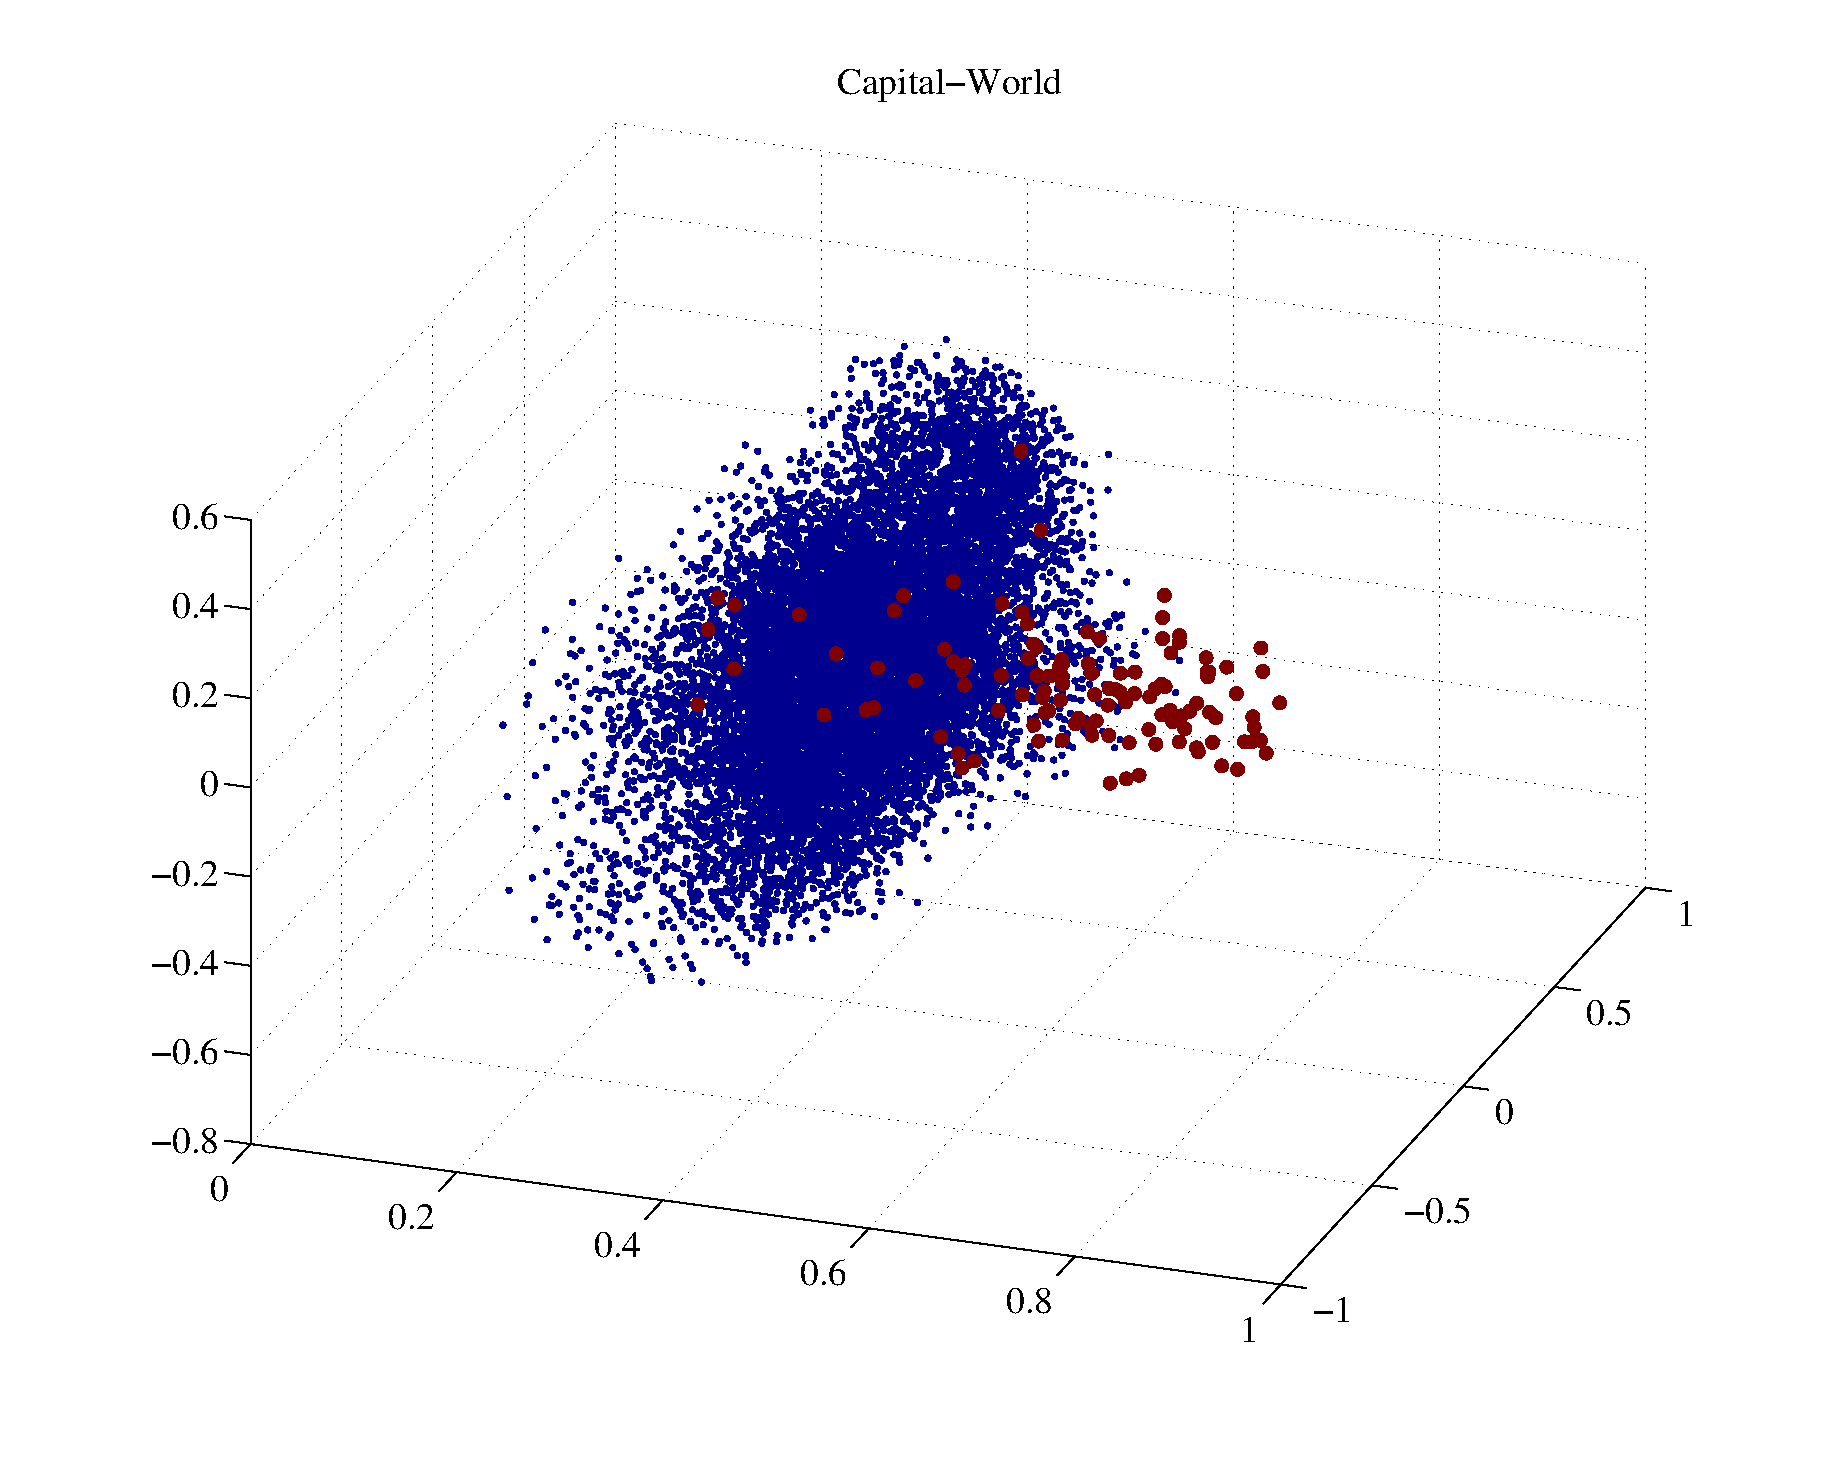
\includegraphics[width=.45\textwidth]{./images/capital_world.eps}
}
\subfigure[Nationality-Adjective]{
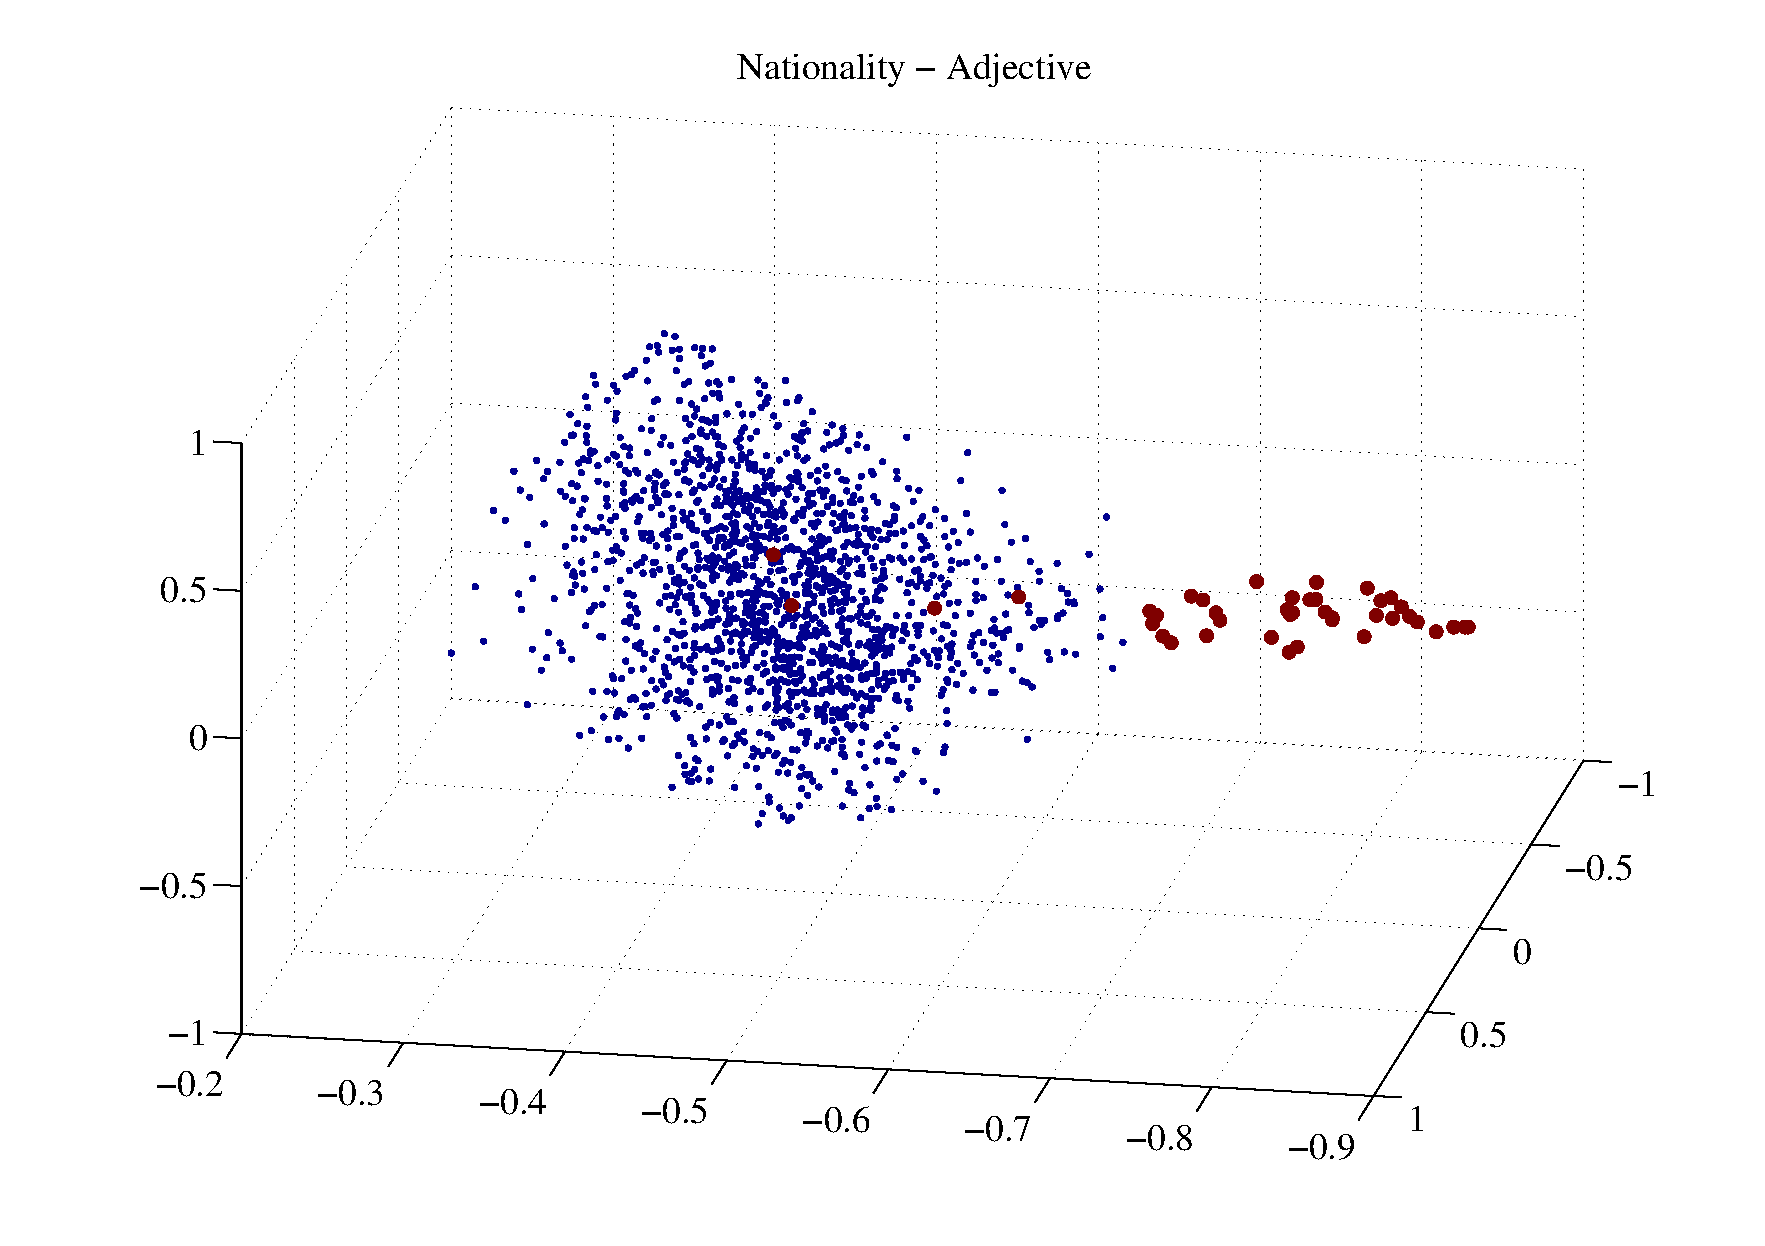
\includegraphics[width=.45\textwidth]{./images/nationality_adj.eps}
}

\subfigure[Plural-Vebs]{
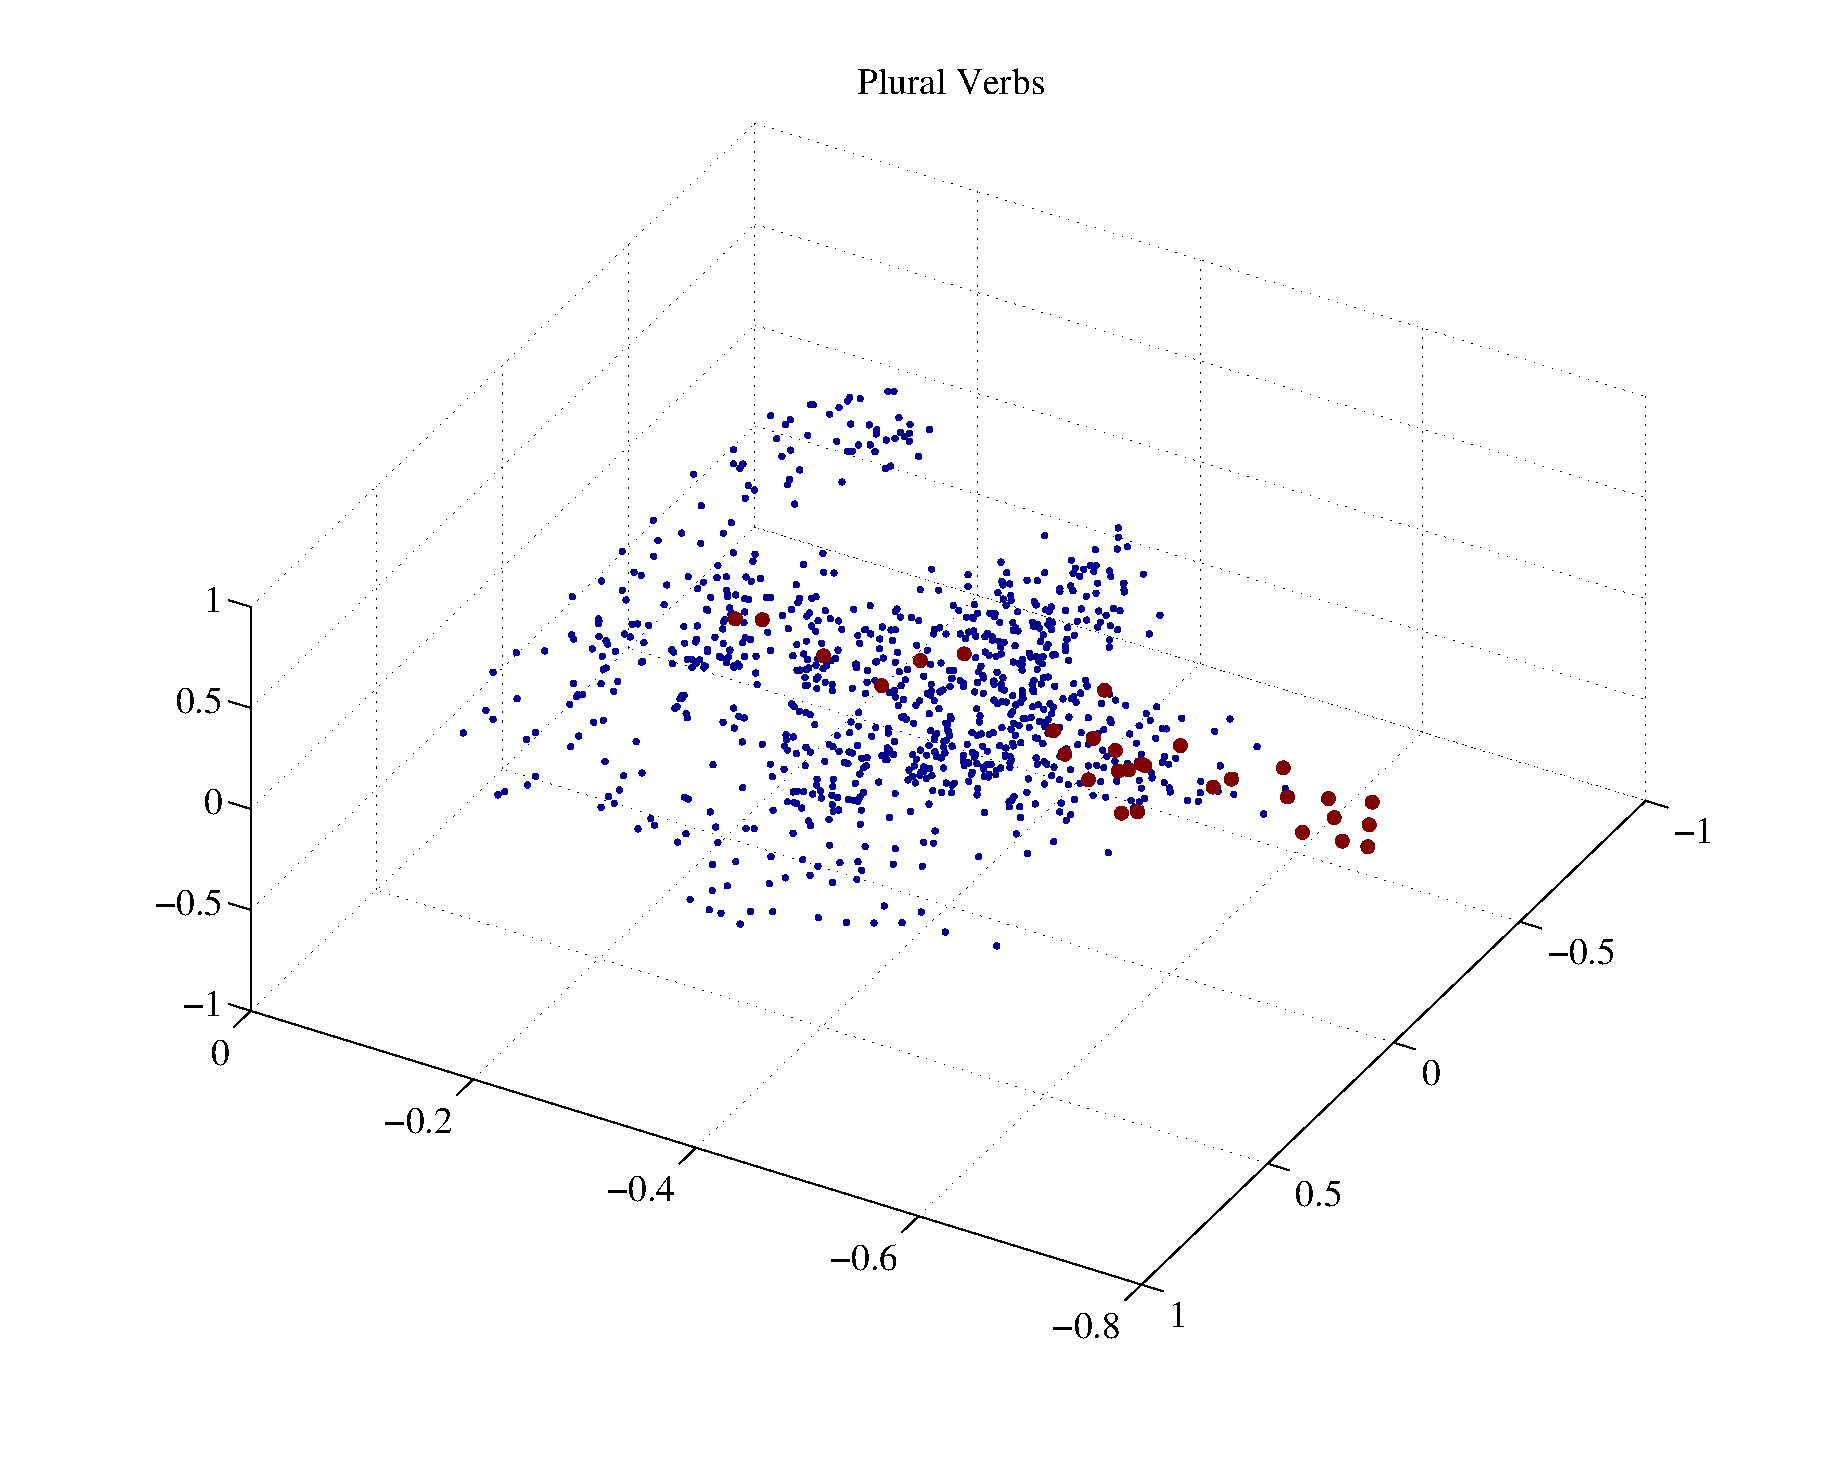
\includegraphics[width=.45\textwidth]{./images/plural_verbs.eps}
}
\caption{Projections of Vector Offsets for different categories of Word-Pairs}
\label{fig:offsetProj}
\end{figure}

\clearpage

\section{Conclusion}
\nocite{*}
\bibliographystyle{splncs}
\bibliography{bibliography}

\end{document}
